\newpage\section{Analysis}

In \autoref{fig:waves}, the evolution of the wave field originating from the initial perturbation can be observed. The solution exhibits radial outward wave propagation, while no clear Coriolis-induced deflection is visible at this timescale. After approximately 12 minutes, the waves reach the domain boundaries, where they are reflected due to the imposed solid wall conditions. Another notable feature is that the waves propagate relatively quickly across the domain, which however is consistent with the chosen parameter values.

\begin{figure}[H]
    \centering
    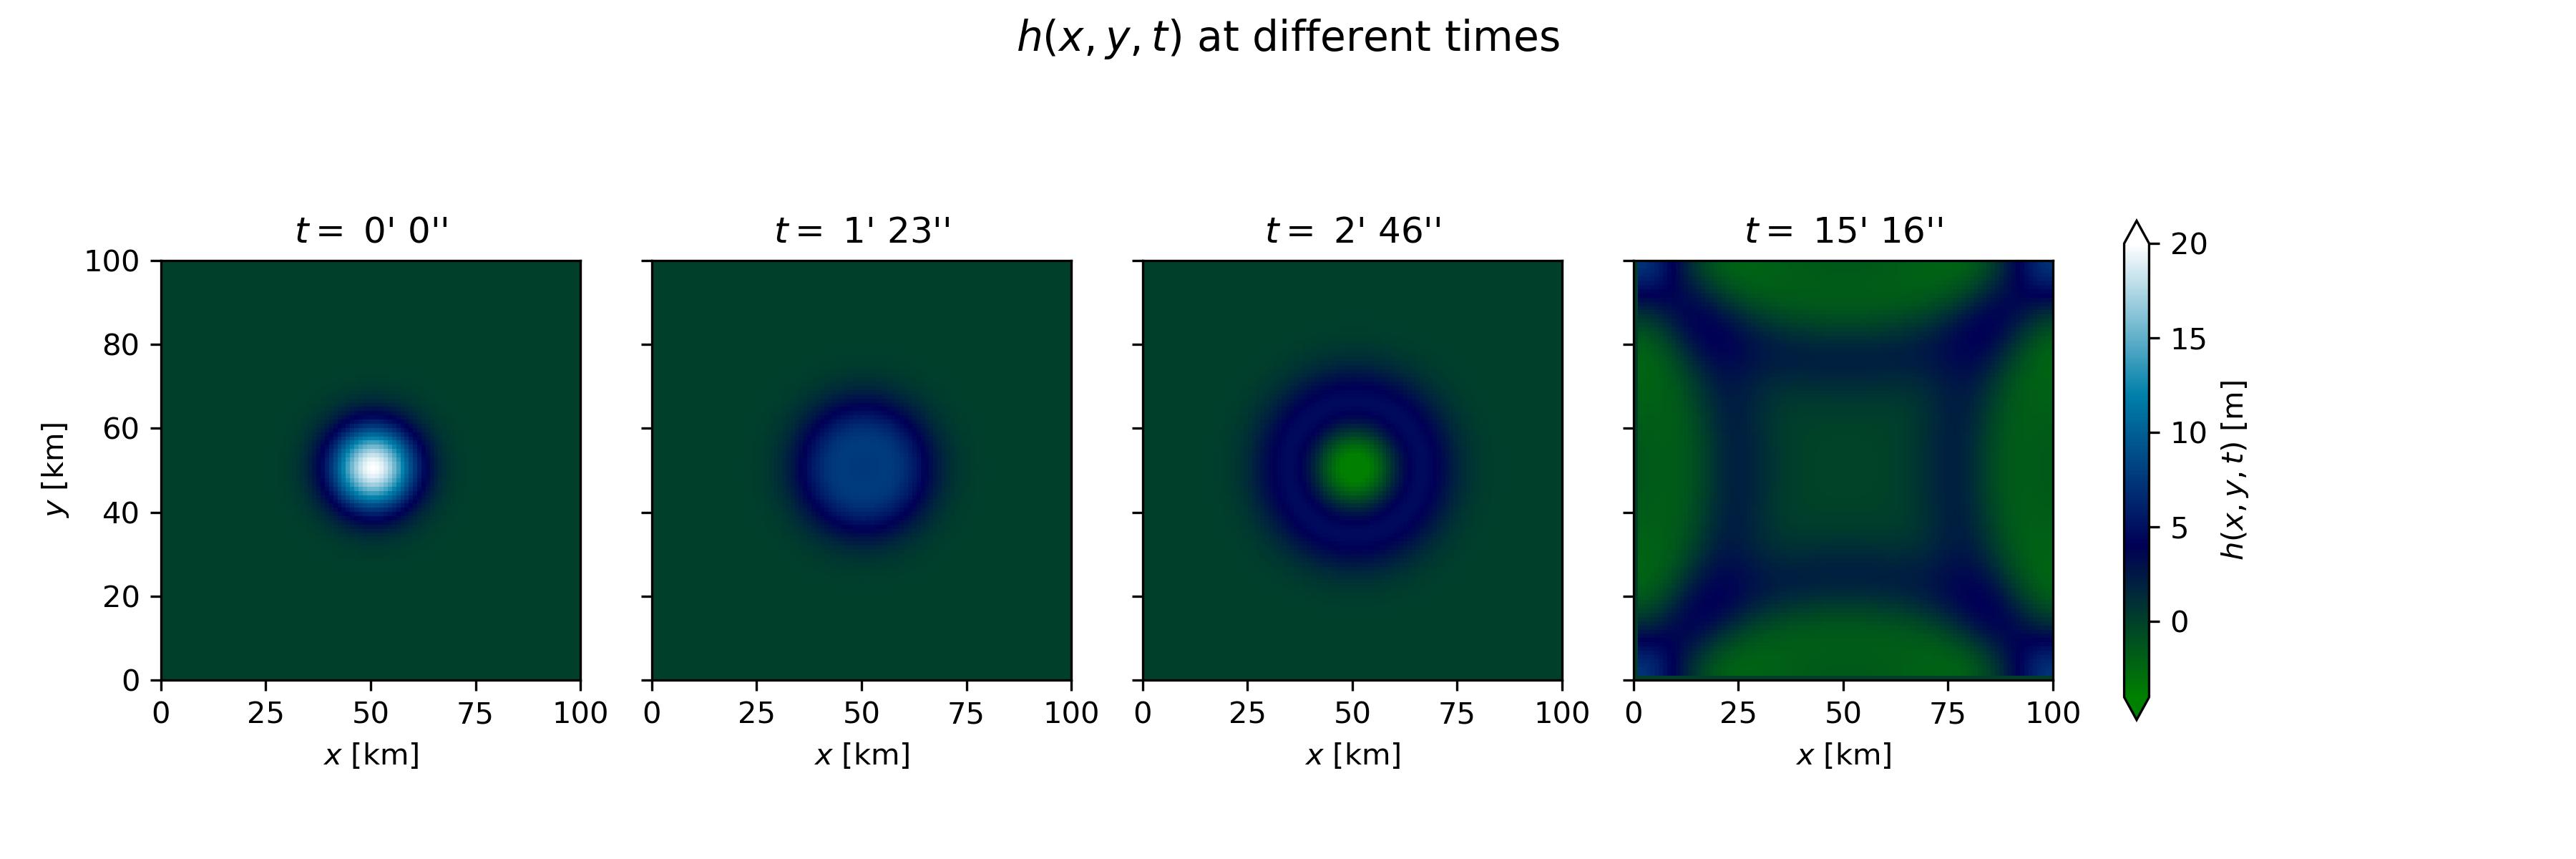
\includegraphics[width=1.1\textwidth]{Figures/ocean-waves.png}
    \caption{Time evolution of the surface height $h(x,y,t)$ showing wave propagation and boundary reflections.}
    \label{fig:waves}
\end{figure}

In \autoref{fig:energy}, the evolution of total energy and volume is shown for the numerical model. The volume remains nearly constant throughout the simulation, indicating good mass conservation. However, the total energy decreases by approximately 25\%, suggesting the presence of numerical dissipation. The time required for the wave to reach the boundary is consistent with the expected propagation speed, occurring at approximately 12 minutes (around 700 seconds), as also visible in the energy evolution plot.

\begin{figure}[H]
    \centering
    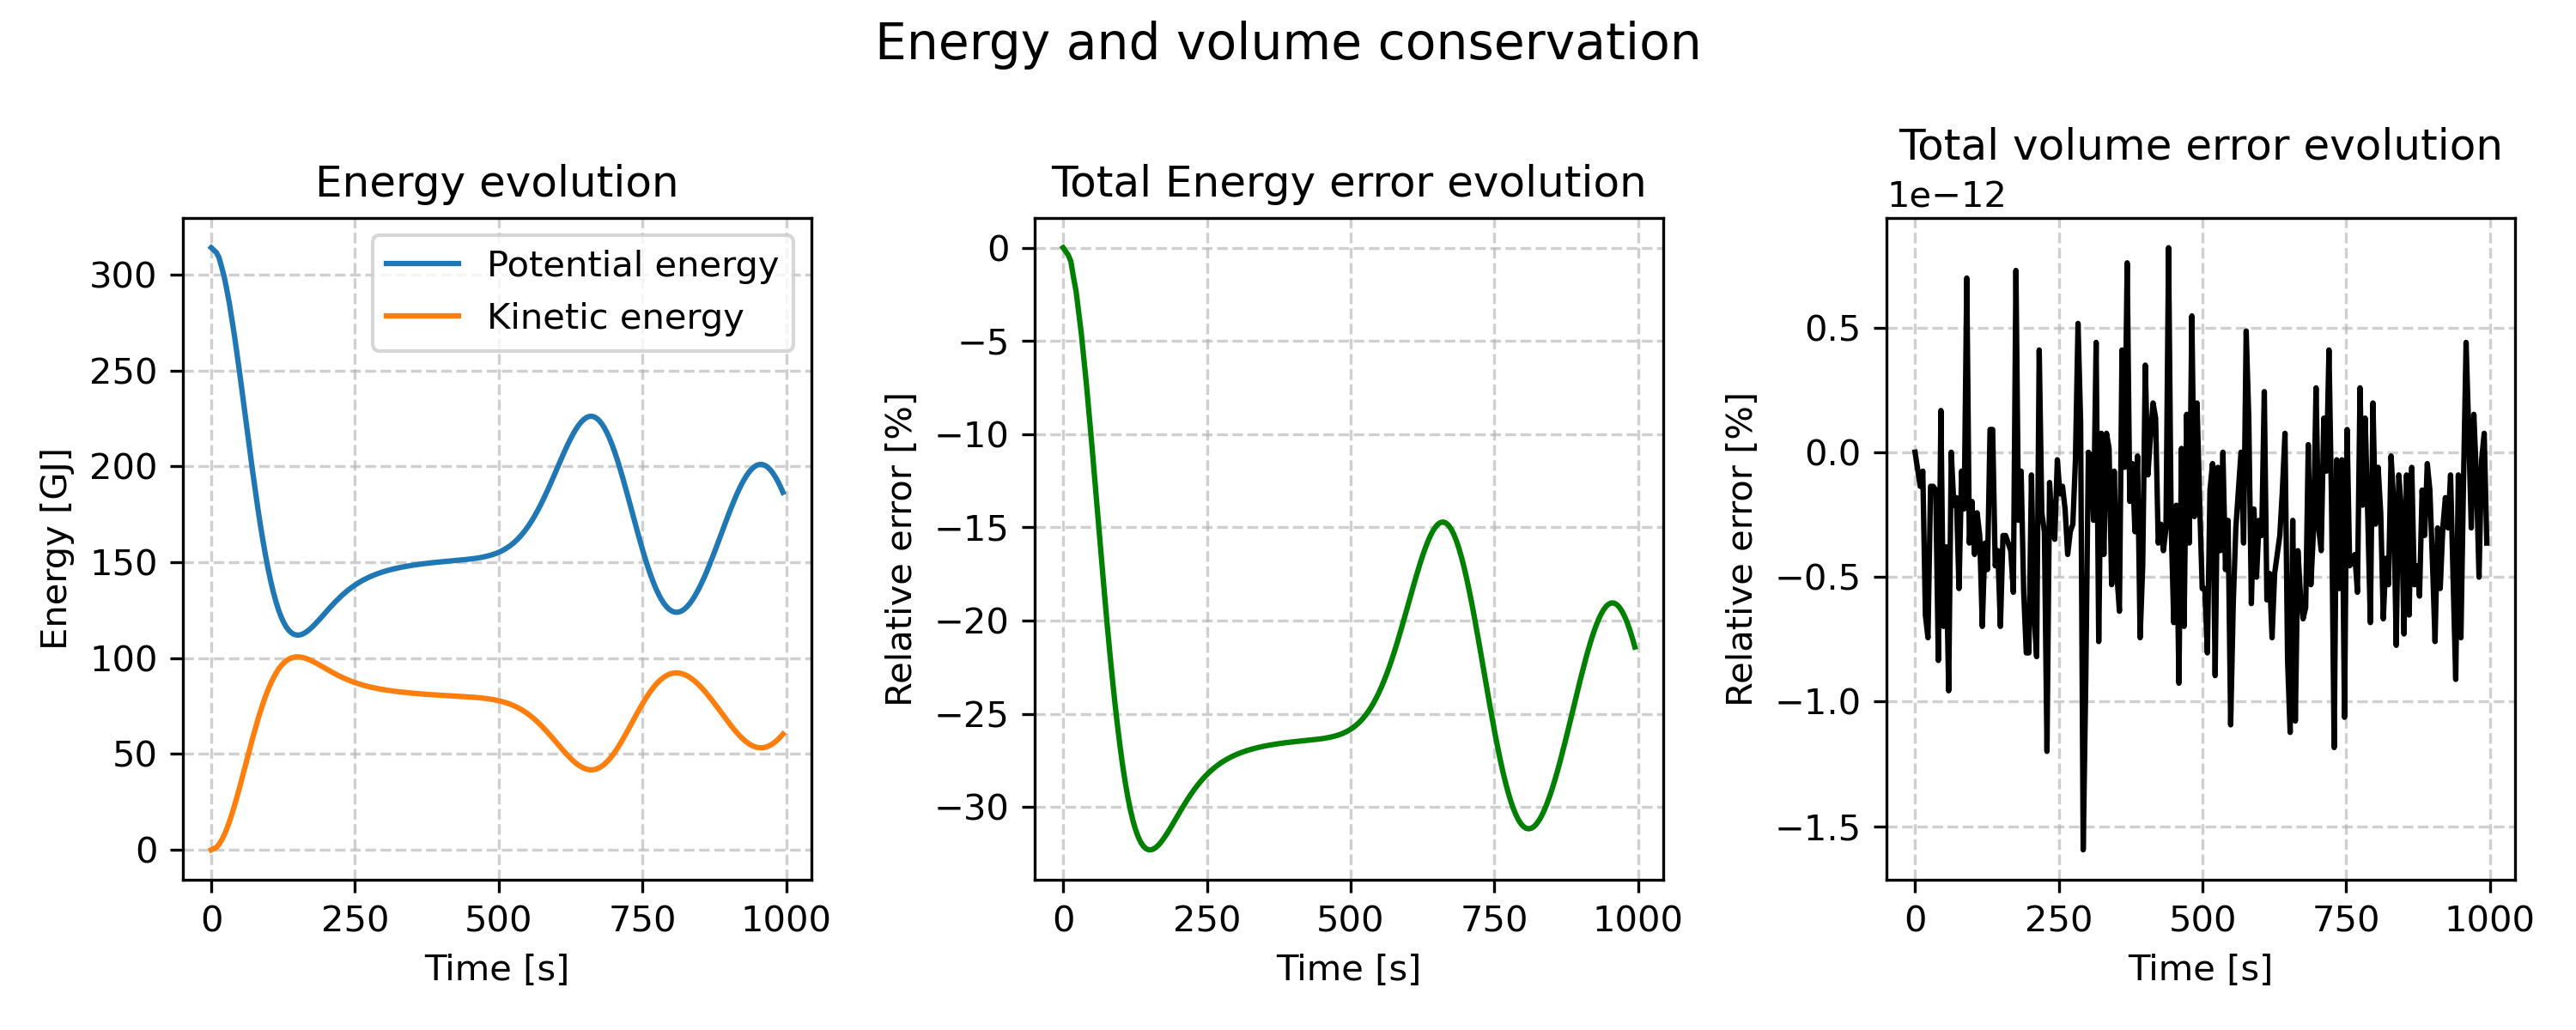
\includegraphics[width=0.8\textwidth]{Figures/energy.png}
    \caption{Time evolution of potential, kinetic, and total energy, showing approximate conservation with minor numerical dissipation.}
    \label{fig:energy}
\end{figure}

The large discrepancy in total energy should be further investigated. The influence of the Robert--Asselin filter was examined, but it does not appear to be the primary source of the energy loss. Similarly, variations in the initial conditions do not significantly affect the observed behaviour. This suggests that the main source of error is likely the initial Forward Euler step used to start the Leapfrog scheme.

This is also consistent with the observation that the largest drop in accuracy occurs at the beginning of the simulation, after which the energy evolution becomes more stable. This indicates that the initial time-stepping procedure may introduce a transient error that is not subsequently amplified by the Leapfrog integration.